\documentclass{article}

\title{Guitar Handbook}
\date{2016-06-18}
\author{Bartek Banachewicz}

\usepackage{tikz}

\begin{document}
\pagenumbering{gobble}
\maketitle
\newpage

\pagenumbering{arabic}
\section{Introduction}
\noindent
This book is aimed to be a guide for intermediate guitarists looking for a quick reference tool in various situations.
Here are the things I'd like to put there:

\subsection{Notes}
The notes section provides information about the individual notes.
\subsection{Intervals}
Extending that to two notes, we get into relationships between two distinct notes, or intervals
\subsection{Scales \& Modes}
By linking together a few intervals, we achieve a scale. My moving the scale root, we form a mode.
\subsection{Chords}
Chords are a huge topic, mostly because they take a concept of scales and extend it to subsets of them played together.

\section{Notes}
\begin{tabular}{ c c c c c c c c }
	A & B & C & D & E & F & G & H \\
	440
\end{tabular}

\begin{tabular}{ c c c c c c c c }
\end{tabular}
\section{Intervals}
\begin{tabular}{ r|c|c }
	Size in half-tones & Name & Alternative name\\
	\hline
	1 & prime & \\
	2 & minor second &\\
	3 & major second & \\
	4 & minor third & \\
	5 & major third & \\
	6 & perfect fourth & diminished fifth \\
	7 & perfect fifth & \\
	8 & minor sixth & augmented fifth \\
	9 & major sixth & \\
	10 & minor seventh & \\
	11 & major seventh & \\
	12 & octave
\end{tabular}
\section{Scales}

\subsection{Scale Square}

\begin{tabular}{ l | *{12}{c|} }
	     & C & C\# & D & D\# & E & F & F\# & G & G\# & A & A\# & B \\
	C    & 1 &     & 2 &     & 3 & 4 &     & 5 &     & 6 &     & 7 \\
	C\#  & 7 &   1 &   &   2 &   & 3 &   4 &   &   5 &   &   6 &   \\
    D    &   &     &   &     &   &   &     &   &     &   &     &   \\
    D\#  &   &     &   &     &   &   &     &   &     &   &     &   \\
    E    &   &     &   &     &   &   &     &   &     &   &     &   \\
    F    &   &     &   &     &   &   &     &   &     &   &     &   \\
    F\#  &   &     &   &     &   &   &     &   &     &   &     &   \\
    G    &   &     &   &     &   &   &     &   &     &   &     &   \\
    G\#  &   &     &   &     &   &   &     &   &     &   &     &   \\
    A    &   &     &   &     &   &   &     &   &     &   &     &   \\
    A\#  &   &     &   &     &   &   &     &   &     &   &     &   \\
    B    &   &     &   &     &   &   &     &   &     &   &     &   \\
   
	
\end{tabular}

\section{Chords}
Chords

\subsection{Major}

\begin{tabular}{ l | r }
Marking      & C, CM, Cmaj \\
Scale        & major \\
Steps        & 1 - 3 - 5 \\
Example in C & C - E - G \\
\end{tabular}

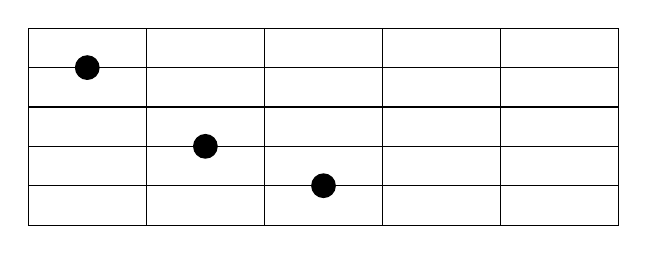
\begin{tikzpicture}[scale=0.5]
% strings
\draw (0,0) rectangle (15,5);
\path[draw] (0,1) -- (15,1);
\path[draw] (0,2) -- (15,2);
\path[draw] (0,3) -- (15,3);
\path[draw] (0,4) -- (15,4);

% frets
\path[draw] (3,0) -- (3,5);
\path[draw] (6,0) -- (6,5);
\path[draw] (9,0) -- (9,5);
\path[draw] (12,0) -- (12,5);


\newcommand\chorddot[2]{ \draw[fill=black] (#2*3 - 1.5, 6-#1) circle (.3); }
% chord
\chorddot{2}{1};
\chorddot{4}{2};
\chorddot{5}{3};
\end{tikzpicture}

\subsection{Minor}

\begin{tabular}{ l | r }
Marking      & Cm, Cmin \\
Scale        & minor \\
Steps        & 1 - 3 - 5 \\
Example in C & C - E$\flat$ - G \\
Intervals    & Prime - Minor 3rd - Fifth \\
\end{tabular}

\subsection{Major 7}
\begin{tabular}{ l | r }
    Marking      & C7, Cmaj7 \\
    Scale        & minor \\
    Steps        & 1 - 3 - 5 - 7 \\
    Example in C & C - E$\flat$ - G \\
    Intervals    & Prime - Minor 3rd - Fifth - Major 7th\\
\end{tabular}

\subsection{Minor 7}
\begin{tabular}{ l | r }
    Marking      & Cm7, Cmin7 \\
    Scale        & minor \\
    Steps        & 1 - 3 - 5 - 7 \\
    Example in C & C - E$\flat$ - G \\
    Intervals    & Prime - Minor 3rd - Fifth - Minor 7th \\
\end{tabular}

\subsection{Augmented}
A major chord with an augmented fifth.

\begin{tabular}{ l | r }
    Marking      & Caug, C+, C+5 \\
    Scale        & minor \\
    Steps        & 1 - 3 - 5 \\
    Example in C & C - E$\sharp$ - G$\sharp$ \\
    Intervals    & Prime - Major 3rd - Augmented Fifth \\
\end{tabular}

\subsection{Diminished}
A minor chord with a diminished fifth.

\begin{tabular}{ l | r }
    Marking      & Cdim, C$^{\circ}$ \\
    Scale        & minor \\
    Steps        & 1 - 3 - 5 \\
    Example in C & C - E$\flat$ - G$\flat$ \\
    Intervals    & Prime - Minor 3rd - Diminished Fifth \\
\end{tabular}


\end{document}